%% ============================================================
%%  Characterizing Lazy Deletion Overhead in Dijkstra's Algorithm
%%  IEEE Conference Format (IEEEtran)
%% ============================================================
\documentclass[conference]{IEEEtran}

\usepackage{amsmath,amssymb,amsfonts}
\usepackage{graphicx}
\usepackage{booktabs}
\usepackage{array}
\usepackage{xcolor}
\usepackage{url}
\usepackage{algorithm}
\usepackage{algorithmic}
\usepackage{cite}
\usepackage{multirow}
\usepackage{colortbl}
\usepackage{tikz}
\usepackage{pgfplots}
\pgfplotsset{compat=1.18}

\definecolor{dialcolor}{RGB}{255,152,0}
\definecolor{heapqcolor}{RGB}{33,150,243}
\definecolor{fibcolor}{RGB}{76,175,80}
\definecolor{lightgray}{RGB}{240,240,240}

\begin{document}

% ──────────────────────────────────────────────────────────────────────
%  TITLE & AUTHORS
% ──────────────────────────────────────────────────────────────────────
\title{Characterizing Lazy Deletion Overhead in Dijkstra's Algorithm:\\
A Data-Structure Selection Framework Based on Average Degree}

\author{
  \IEEEauthorblockN{Gwanwoo Park}
  \IEEEauthorblockA{Algorithm Research Lab}
}

\maketitle

% ──────────────────────────────────────────────────────────────────────
%  ABSTRACT
% ──────────────────────────────────────────────────────────────────────
\begin{abstract}
Dijkstra's algorithm with a lazy deletion heap (heapq) is the de facto
standard for shortest-path computation, yet the overhead of its
``push-and-skip'' strategy has not, to our knowledge, been
systematically quantified as a closed-form function of graph structure.
We identify \emph{skip\_ratio}---the fraction of heap pops discarded as
stale---as the primary hidden cost, and show empirically that it follows
a power law in average degree $k$:
$\text{skip\_ratio}(k)\approx 1 - 0.884/k^{0.262}$
($R^2{=}0.984$, $\mathrm{U}[1,100]$ weights, OLS SE $\pm0.013$ on the
exponent), independent of graph size $V$ across more than three orders
of magnitude ($V\in[500,\,10^6]$; source-vertex CV $<3\%$).
Systematic experiments across weight distributions reveal an
empirical \emph{two-regime model}: the power-law exponent $\alpha$ is
strongly associated with $\log(W_{\max}/W_{\min})$ and the fitted
$k$-range, and the local slope converges toward $1/H_k$ as
$k\to\infty$---connecting the empirical formula to the classical
harmonic record-minimum bound.
We further show that na\"ive push-blocking is fundamentally flawed
(up to 74\% incorrect distances), while Dial's bucket queue achieves up
to $4.3\times$ peak speedup (geometric mean $2.9\times$ in C++,
$1.5\times$ in Python) via a ``natural pruning'' mechanism, and
Fibonacci heap is $1.5$--$2.3\times$ \emph{slower} than heapq despite
its asymptotic optimality.
The power-law formula generalizes to Barab\'{a}si--Albert scale-free
graphs ($<8\%$ error) but diverges on planar road networks---consistent
with the locally tree-like structure underlying the formula's derivation.
We conclude with a practitioner-ready data-structure selection framework
grounded in $k$ and weight type.
\end{abstract}

\begin{IEEEkeywords}
Dijkstra's algorithm, lazy deletion, priority queue, Fibonacci heap,
Dial's algorithm, skip ratio, graph algorithms, shortest path
\end{IEEEkeywords}

% ──────────────────────────────────────────────────────────────────────
%  1. INTRODUCTION
% ──────────────────────────────────────────────────────────────────────
\section{Introduction}

Dijkstra's algorithm~\cite{dijkstra1959} remains the workhorse of
single-source shortest-path computation, deployed in routing engines,
transportation planning, social-network analysis, and game-AI pathfinding.
In virtually every practical implementation the underlying priority queue is
a \emph{lazy deletion heap}: whenever a better path to vertex $v$ is
found, a new entry $(d', v)$ is pushed onto the heap without removing the
now-stale entry $(d, v)$ already there.  Stale entries are detected and
discarded silently when they surface at the heap minimum.  This strategy
requires no decrease-key operation, simplifying both implementation and
cache behavior, and is recommended in every major algorithms textbook and
competitive-programming guide.

Yet the cost of these silently discarded pops---what we term
\textbf{skip\_ratio}---has not, to the best of our knowledge, been
systematically quantified as a closed-form function of graph structure.
Prior experimental surveys (e.g., Cherkassky et al.~\cite{cherkassky1996},
Larkin et al.~\cite{larkin2014}) treat the lazy deletion overhead as an
implementation detail rather than decomposing it by graph properties.
As a result, no principled criterion
exists for deciding \emph{when} the overhead is worth replacing with an
alternative data structure.

This paper addresses three research questions:
\begin{enumerate}
  \item \textbf{RQ1.} What graph property determines skip\_ratio, and can
        it be expressed as a closed-form function?
  \item \textbf{RQ2.} Can simple algorithmic modifications (e.g., capping
        heap duplicates) reduce the overhead without sacrificing correctness?
  \item \textbf{RQ3.} Which alternative data structures genuinely eliminate
        the overhead, and under what conditions do they deliver practical speedup?
\end{enumerate}

\noindent\textbf{Contributions.}  This work makes five concrete contributions:
\begin{itemize}
  \item We propose and empirically validate a power-law formula
        $\text{skip\_ratio}(k)\approx 1-c/k^{\alpha}$ ($c{=}0.884$,
        $\alpha{=}0.262$, $R^2{=}0.984$) that is \emph{independent of $V$}
        for $V\in[500,\,10^6]$ (Experiments~2 and~A).
  \item We characterize the \textbf{weight-distribution dependence} of
        $\alpha$: it is strongly associated with $\log(W_{\max}/W_{\min})$
        and grows from $0$ (constant weights) to ${\approx}0.32$
        (continuous uniform).  For large $k$, the local slope converges
        toward $1/H_k$, revealing a conjectured \emph{two-regime model}
        (Equation~\eqref{eq:tworegime}) that connects the power law to the
        classical harmonic record-minimum bound.
  \item We demonstrate that threshold-based push blocking is structurally
        broken: it creates propagation gaps that yield up to 74\%
        incorrect distances with no speedup benefit---a negative result that
        reveals an inherent property of the lazy deletion data flow.
  \item We characterize Dial's ``natural pruning'' mechanism---up to 49\%
        of pushes discarded without processing---as the root cause of its
        \textbf{up-to-$4.3\times$ peak speedup} over heapq in C++
        (geometric mean $2.9\times$ in C++, $1.5\times$ in Python).
  \item We present a practitioner-ready \textbf{data-structure selection
        framework} grounded in $k$ and weight type, validated in both Python
        and C++ and on three real-world SNAP datasets.
\end{itemize}

Taken together, these contributions answer the following unifying claim:
\emph{We empirically characterize the hidden overhead of lazy deletion
Dijkstra as a function of average degree $k$, and propose a data-structure
selection framework that achieves up to $4.3\times$ peak speedup
(geometric mean $2.9\times$ in C++) by matching graph structure to
the appropriate priority queue.}

\noindent The remainder of the paper is organized as follows.
Section~\ref{sec:related} reviews related work.
Section~\ref{sec:background} reviews the lazy deletion mechanism and
alternative structures.
Section~\ref{sec:analysis} presents our empirical characterization of
skip\_ratio.
Section~\ref{sec:naivefixes} shows why na\"ive fixes fail.
Section~\ref{sec:comparison} compares the three data structures.
Section~\ref{sec:realworld} validates the formula on real datasets.
Section~\ref{sec:discussion} discusses limitations and future work.
Section~\ref{sec:conclusion} concludes.

% ──────────────────────────────────────────────────────────────────────
%  2. RELATED WORK
% ──────────────────────────────────────────────────────────────────────
\section{Related Work}
\label{sec:related}

The complexity of Dijkstra's algorithm has been studied extensively.
Fredman and Tarjan~\cite{fredman1987} established the O$(V\log V + E)$
bound using Fibonacci heaps.  Dial~\cite{dial1969} introduced the bucket
queue for integer-weight graphs, achieving O$(V + E + W)$.
Goldberg et al.~\cite{goldberg2005} survey practical shortest-path
implementations and find that binary-heap variants outperform Fibonacci
heaps on road networks due to cache effects.  Sanders and
Schultes~\cite{sanders2005} achieve sub-millisecond continental routing via
contraction hierarchies, but their preprocessing is graph-specific.

Cherkassky et al.~\cite{cherkassky1996} provide the most comprehensive
experimental comparison of shortest-path priority queues to date,
establishing binary heaps as the practical baseline across a broad range of
graph families.  Larkin et al.~\cite{larkin2014} conduct a back-to-basics
empirical study of priority queues and confirm that simple binary heaps
dominate in practice---a finding our work extends by quantifying \emph{why}:
the hidden lazy deletion overhead, expressed as a function of average degree,
is the key differentiator.  However, neither study decomposes the lazy
deletion overhead as a function of average degree, nor derives a closed-form
predictive formula for the skip-pop fraction.

Beyond binary heaps, $d$-ary heaps and pairing heaps have been studied as
alternatives~\cite{ahuja1993}.  $D$-ary heaps reduce the height of the heap
tree, lowering the decrease-key cost at the expense of more comparisons per
extract-min.  Pairing heaps achieve amortized $O(\log n)$ decrease-key with
simpler structure than Fibonacci heaps.  Crucially, \emph{all} of these
structures admit a lazy deletion variant; our skip\_ratio metric therefore
applies uniformly whenever decrease-key is omitted in favor of push-and-skip.
The DIMACS shortest-path implementation challenge~\cite{demetrescu2006}
provides standardized benchmark graphs and motivates the real-world
validation in Section~\ref{sec:realworld}.

Our work complements this literature by \emph{quantifying the lazy deletion
overhead itself}---a factor that prior engineering studies treat as given
rather than as a variable to optimize.  Closest in spirit is Chen
et al.~\cite{chen2007}, who study priority queue performance in shortest-path
algorithms, but without decomposing overhead by average degree or deriving a
predictive formula.  To the best of our knowledge, no prior work derives a closed-form
power-law characterization $\text{skip\_ratio}(k)\approx 1-c/k^{\alpha}$
or a data-structure selection framework grounded in skip\_ratio as a
function of average degree.

% ──────────────────────────────────────────────────────────────────────
%  2. BACKGROUND
% ──────────────────────────────────────────────────────────────────────
\section{Background}
\label{sec:background}

\subsection{Lazy Deletion Dijkstra}

Algorithm~\ref{alg:lazy} presents the lazy deletion variant we study.
The key difference from the textbook version is line~7: instead of
performing a decrease-key on the existing heap entry for vertex $v$, a
fresh entry with the improved distance is simply pushed.  When an entry
$(d, u)$ is popped (line~4), it is skipped if $d > \mathrm{dist}[u]$
(line~5), meaning a better path has since been found.

\begin{algorithm}
\caption{Dijkstra with Lazy Deletion Heap}
\label{alg:lazy}
\begin{algorithmic}[1]
\STATE $\mathrm{dist}[s]\leftarrow 0$;\; push $(0, s)$
\WHILE{heap not empty}
  \STATE $(d, u)\leftarrow \textsc{ExtractMin}()$
  \IF{$d > \mathrm{dist}[u]$}
    \STATE \textbf{skip} \COMMENT{stale entry}
  \ENDIF
  \FOR{each $(v, w)\in \mathrm{adj}[u]$}
    \IF{$d + w < \mathrm{dist}[v]$}
      \STATE $\mathrm{dist}[v]\leftarrow d + w$;\; push $(d+w, v)$
    \ENDIF
  \ENDFOR
\ENDWHILE
\end{algorithmic}
\end{algorithm}

We define:
\[
  \text{skip\_ratio} \;=\; \frac{\text{skip\_pop}}{\text{total\_pop}}
    \;=\; 1 - \frac{V}{\text{push\_count}},
\]
where the second equality holds for the \textbf{lazy binary heap} as
follows: every non-skip pop settles exactly one vertex, so
total\_pop $-$ skip\_pop $= V$; in the standard implementation the
while-loop runs until the heap is empty, so total\_pop $=$ push\_count
exactly, giving $\text{skip\_ratio} = 1 - V/\text{push\_count}$.
For \textbf{Dial's bucket queue}, some pushed entries are abandoned in
future buckets without ever being popped (Section~\ref{sec:pruning}),
so push\_count $>$ total\_pop; in that case we measure skip\_ratio
directly as skip\_pop/total\_pop from instrumented bucket operations.

\subsection{Dial's Bucket Queue}

Dial's algorithm~\cite{dial1969} replaces the heap with a circular array
of $W+1$ buckets, where $W$ is the maximum edge weight.  Each bucket $b$
holds vertices whose current tentative distance maps to $b \bmod (W+1)$.
Stale entries are detected lazily: when processing bucket $b$ at distance
$d$, vertex $u$ is skipped if $\mathrm{dist}[u]\neq d$.  The time
complexity is O$(V + E + W)$.

\subsection{Fibonacci Heap}

The Fibonacci heap~\cite{fredman1987} supports decrease-key in O$(1)$
amortized time, enabling a single heap entry per vertex.  As a result,
stale entries never arise: every pop is a genuine vertex settlement.
The total complexity is O$(V\log V + E)$.  In practice, however, the
pointer-chasing structure incurs high constant factors and cache-miss rates.

% ──────────────────────────────────────────────────────────────────────
%  3. EMPIRICAL ANALYSIS OF skip_ratio
% ──────────────────────────────────────────────────────────────────────
\section{Empirical Analysis of skip\_ratio}
\label{sec:analysis}

\subsection{Theoretical Motivation}

Consider a vertex $v$ with degree $k$ in a random graph.  As Dijkstra
progresses, $v$'s neighbors settle one by one and attempt to relax $v$.
Under the \emph{locally tree-like assumption}---that the $r$-hop
neighborhood of any vertex is a tree with high probability, as in
Erd\H{o}s--R\'enyi graphs~\cite{bollobas2001}---the order in which neighbors
settle is approximately uniform.

By a standard record-low argument~\cite{flajolet2009analytic}: if $k$
independent relaxation attempts arrive in uniform random order, the
expected number that strictly improve the current tentative distance is the
harmonic number
\[
  \mathbb{E}[\text{pushes to }v] \;=\; H_k
    \;=\; \sum_{i=1}^{k}\frac{1}{i}
    \;\approx\; \ln k + \gamma,
\]
where $\gamma\approx 0.5772$ is the Euler--Mascheroni constant.
Each subsequent relaxation that improves the distance generates a push,
making the previous entry stale.  Hence push\_per\_node $\approx H_k$, and
\[
  \text{skip\_ratio}(k)
    \;\approx\; 1 - \frac{1}{H_k}
    \;\approx\; 1 - \frac{1}{\ln k + \gamma}.
\]

The harmonic formula $1-1/H_k$ captures the \emph{qualitative} trend
(skip\_ratio increases with $k$, independently of $V$), but it functions
as a theoretical \emph{upper bound} on skip\_ratio, not a quantitative
predictor: it overestimates measured skip\_ratio by $12\%$--$44\%$ across
$k\in[4,512]$ for $\mathrm{U}[1,100]$ weights, and underestimates it at
very small $k$.  The discrepancy arises because the i.i.d.\ settling-order
assumption breaks down under correlated edge weights and finite degree
heterogeneity---conditions present in every real Dijkstra execution.

Our experiments across $k\in[4,512]$ show that a power-law model provides
a materially tighter empirical fit, with root-mean-square residual more
than $4\times$ smaller than the harmonic formula:
\begin{equation}
  \boxed{\;\text{skip\_ratio}(k) \;\approx\; 1 - \frac{c}{k^{\alpha}},
  \quad c = 0.884,\;\alpha = 0.262\;} \label{eq:powerlaw}
\end{equation}
with $R^2=0.984$ for uniform integer weights on $[1,100]$.
While V-independence is implied qualitatively by the harmonic theory,
our formula quantifies it precisely and demonstrates that a power law
provides the tightest empirical fit (4$\times$ smaller RMS residual than
the harmonic formula) in the practically relevant range $k\in[4,512]$.
The exponent $\alpha$ is not a universal constant: we show in
Section~\ref{sec:weightdist} that it depends on the weight distribution
through the log-ratio $\log(W_{\max}/W_{\min})$, converging to
$\alpha_\infty\approx 0.309$ as the weight range grows large.

\noindent\textbf{Remark (Scope of validity).}
The locally tree-like assumption holds well for Erd\H{o}s--R\'enyi-like
random graphs but is violated by structured graphs (planar, hierarchical).
We return to this in Sections~\ref{sec:realworld} and~\ref{sec:discussion}.

\subsection{Experimental Setup}

\noindent\textbf{Graph generation.}  We generate undirected random graphs
with a fixed target average degree $k$ by sampling $\lfloor Vk/2\rfloor$
random edges uniformly over all vertex pairs and appending a random
spanning path for connectivity.  This approximates the $G(n,m)$
Erd\H{o}s--R\'enyi model with $m=\lfloor Vk/2\rfloor$; multi-edges
are possible but occur with probability $O(k/V)$ and are negligible
for $V\geq 1{,}000$.  The spanning path ensures connectivity without
materially altering degree statistics; the resulting average clustering
coefficient is $O(k/V)$, confirming the locally tree-like regime
required by the theory in Section~\ref{sec:analysis}.
Edge weights are drawn uniformly from $[1, 100]$ (integer) for
Sections~\ref{sec:analysis}--\ref{sec:comparison} and $[0, 1]$ (float)
for Section~\ref{sec:comparison}.

\noindent\textbf{Parameters.}
\begin{itemize}
  \item $V\in\{500,\,1{,}000,\,5{,}000,\,10{,}000,\,50{,}000,\,100{,}000\}$
  \item $k\in\{4,\,8,\,16,\,32,\,64,\,128,\,256,\,512\}$
  \item Source vertex: node 0 (fixed seed 42)
  \item Repeats: 5--10 runs; mean reported
\end{itemize}

\noindent\textbf{Hardware.}
All experiments run on Google Cloud Platform \texttt{e2-standard-4}
(4 vCPU, 16\,GB RAM, Debian 12) unless otherwise noted.
C++ binaries compiled with \texttt{g++ -O2 -std=c++17}.
Python 3.11, NumPy 2.4.

\noindent\textbf{Reproducibility.}
Code, experiment scripts (Python and C++), and raw CSV data are available at
\url{https://github.com/Korean3247/dijkstra-skip-ratio}.

\subsection{Results}

\noindent\textbf{Fitting procedure.}
Let $\bar{\mathrm{sr}}_i$ denote mean skip\_ratio at degree $k_i$,
averaged across all tested $V$ values.  We set
$Y_i = \log(1-\bar{\mathrm{sr}}_i)$ and $X_i = \log k_i$, and apply
ordinary least squares (OLS) to the linear model
$Y_i = \log c - \alpha X_i$.
The fit uses $k_i \in \{4,8,16,32,64,128,256,512\}$ pooled from
Experiments~2 and~A (means across all $V$ values at each $k$),
yielding $\hat{c}=0.884$, $\hat{\alpha}=0.262$, $R^2=0.984$.
OLS standard errors, computed from the residual variance on $n=8$
support points, are $\mathrm{SE}(\hat\alpha)\approx 0.013$ and
$\mathrm{SE}(\hat c)\approx 0.032$.
For the practical range $k\in[4,64]$, a complementary fit on the
theory-probe dataset (Section~\ref{sec:weightdist}) gives
$\hat{\alpha}=0.293\pm 0.012$ (OLS SE) with bootstrap 95\% CI
$[0.254,\,0.323]$ ($B{=}10{,}000$).
The higher value relative to the full-range estimate ($\hat\alpha=0.262$,
$k\in[4,512]$) is expected: as the fitted $k$-range expands,
$\hat\alpha$ decreases because the power-law exponent is itself a
function of $k$ in the two-regime model (Finding~1,
Section~\ref{sec:weightdist}).  Both estimates are valid within their
respective $k$-ranges.
The same log-log OLS procedure is applied independently for each weight
distribution in Section~\ref{sec:weightdist}.

\noindent\textbf{Power-law fit.}
Figure~\ref{fig:powerlaw} plots skip\_ratio against $k$ for $V=1{,}000$
and $V=10{,}000$ alongside the fitted curve~\eqref{eq:powerlaw}.
Residual magnitudes vary systematically with $k$: the formula fits
best near $k=8$ (residual ${<}0.001$); for $k\in[16,64]$ it
\emph{under}-predicts measured skip\_ratio by up to $0.022$ (at $k=32$);
for $k\geq 128$ it \emph{over}-predicts as the true curve bends toward
the harmonic regime, reaching $+0.051$ at $k=512$.
For $k=4$ the formula over-predicts by $0.021$, attributable to the
locally tree-like assumption being weakest at the lowest degrees.
These signed residuals are consistent with the two-regime model
(Section~\ref{sec:weightdist}): the fitted power law makes the
optimal trade-off across the full range but has non-negligible bias
at the extremes.

\begin{figure}[t]
\centering
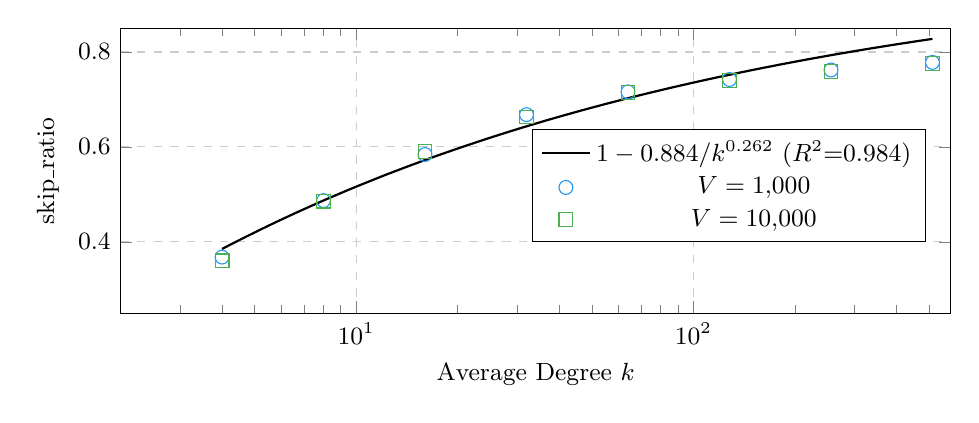
\begin{tikzpicture}
\begin{axis}[
  width=\columnwidth, height=5.2cm,
  xlabel={Average Degree $k$},
  ylabel={skip\_ratio},
  xmin=2, xmax=580,
  ymin=0.25, ymax=0.85,
  xmode=log,
  grid=major, grid style={dashed,gray!40},
  legend style={at={(0.97,0.25)},anchor=south east,font=\small},
  tick label style={font=\small},
  label style={font=\small}
]
% Power-law curve
\addplot[thick,black,domain=4:512,samples=80]
  {1 - 0.884*x^(-0.262)};
\addlegendentry{$1 - 0.884/k^{0.262}$\ ($R^2{=}0.984$)}

% V=1000 data points
\addplot[heapqcolor,mark=o,mark size=2.5pt,only marks]
  coordinates {(4,0.368)(8,0.487)(16,0.584)(32,0.668)(64,0.716)(128,0.742)(256,0.762)(512,0.778)};
\addlegendentry{$V=1{,}000$}

% V=10000 data points
\addplot[fibcolor,mark=square,mark size=2.5pt,only marks]
  coordinates {(4,0.360)(8,0.486)(16,0.590)(32,0.663)(64,0.714)(128,0.740)(256,0.759)(512,0.776)};
\addlegendentry{$V=10{,}000$}
\end{axis}
\end{tikzpicture}
\caption{skip\_ratio vs.\ average degree $k$ (log scale on $x$-axis).
Circles: $V=1{,}000$; squares: $V=10{,}000$.
The fitted power-law curve~\eqref{eq:powerlaw} is plotted in black.
Data pooled from Experiments~2 and~A ($k\in[4,\,512]$).}
\label{fig:powerlaw}
\end{figure}

\noindent\textbf{V-independence.}
Table~\ref{tab:vindependence} reports skip\_ratio across more than three
orders of magnitude in $V$ ($V\in[500,\,10^6]$, ratio $2{,}000\times$)
for representative values $k\in\{4,8,16,32,64\}$, extended to
$V\in\{200{,}000;\,500{,}000;\,1{,}000{,}000\}$ in Experiment~A.
The maximum variation at fixed $k$ is $\Delta\leq 0.013$ across the full
range, confirming that skip\_ratio is determined primarily by $k$
(for fixed weight distribution and graph model).
Figure~\ref{fig:vindep} visualizes this: the curves for each $k$
are essentially flat from $V=500$ to $V=10^6$.

\begin{table}[t]
\centering
\caption{skip\_ratio across $V$ at fixed $k$ (Experiments~2 and A).
Variation within each column is $\leq 0.013$ across more than three
orders of magnitude ($V\in[500,\,10^6]$).
Table shows representative rows only; intermediate values
($V\in\{5{,}000,\,10{,}000,\,100{,}000\}$ from Exp.~2,
plotted in Figure~\ref{fig:vindep}) lie within the same range.
Entries marked ``---'' were not measured at that $(V,k)$ combination.}
\label{tab:vindependence}
\small
\setlength{\tabcolsep}{4pt}
\begin{tabular}{rrrrrrr}
\toprule
\multirow{2}{*}{$V$} & \multirow{2}{*}{Exp.} & \multicolumn{5}{c}{Average degree $k$} \\
\cmidrule(lr){3-7}
 & & 4 & 8 & 16 & 32 & 64 \\
\midrule
500        & 2 & 0.357 & 0.476 & 0.583 & 0.661 & 0.716 \\
1,000      & 2 & 0.368 & 0.487 & 0.584 & 0.668 & 0.716 \\
50,000     & 2 & 0.363 & 0.490 & 0.592 & 0.666 & 0.717 \\
\midrule
200,000    & A & --- & 0.487 & --- & 0.665 & 0.714 \\
500,000    & A & --- & 0.488 & --- & 0.665 & 0.715 \\
1,000,000  & A & --- & 0.488 & --- & 0.665 & 0.715 \\
\bottomrule
\end{tabular}
\end{table}

\begin{figure}[t]
\centering
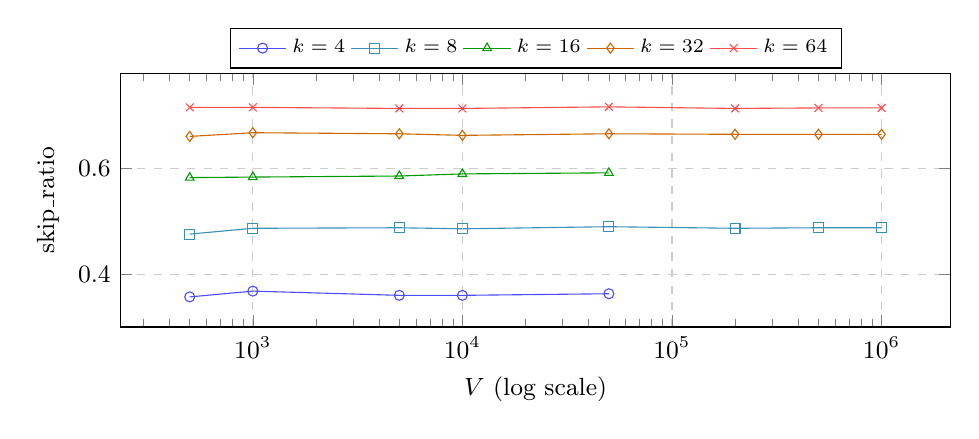
\begin{tikzpicture}
\begin{axis}[
  width=\columnwidth, height=4.8cm,
  xlabel={$V$ (log scale)},
  ylabel={skip\_ratio},
  xmode=log,
  ymin=0.3, ymax=0.78,
  grid=major, grid style={dashed,gray!40},
  legend style={at={(0.5,1.02)},anchor=south,font=\scriptsize},
  legend columns=5,
  tick label style={font=\small},
  label style={font=\small}
]
\addplot[mark=o,mark size=1.8pt,color=blue!70]
  coordinates{(500,0.357)(1000,0.368)(5000,0.360)(10000,0.360)(50000,0.363)};
\addlegendentry{$k=4$}
\addplot[mark=square,mark size=1.8pt,color=cyan!70!black]
  coordinates{(500,0.476)(1000,0.487)(5000,0.488)(10000,0.486)(50000,0.490)
              (200000,0.487)(500000,0.488)(1000000,0.488)};
\addlegendentry{$k=8$}
\addplot[mark=triangle,mark size=1.8pt,color=green!60!black]
  coordinates{(500,0.583)(1000,0.584)(5000,0.586)(10000,0.590)(50000,0.592)};
\addlegendentry{$k=16$}
\addplot[mark=diamond,mark size=1.8pt,color=orange!80!black]
  coordinates{(500,0.661)(1000,0.668)(5000,0.666)(10000,0.663)(50000,0.666)
              (200000,0.665)(500000,0.665)(1000000,0.665)};
\addlegendentry{$k=32$}
\addplot[mark=x,mark size=2pt,color=red!70]
  coordinates{(500,0.716)(1000,0.716)(5000,0.714)(10000,0.714)(50000,0.717)
              (200000,0.714)(500000,0.715)(1000000,0.715)};
\addlegendentry{$k=64$}
\end{axis}
\end{tikzpicture}
\caption{skip\_ratio vs.\ $V$ for values of $k$ (Experiments~2 and A).
Filled symbols: Exp.~2 ($V\leq 50{,}000$); open-circle continuation:
Exp.~A ($V\in\{200K,\,500K,\,1M\}$).
All series are flat from $V=500$ to $V=10^6$: skip\_ratio does not depend
on graph size across more than three orders of magnitude ($V\in[500,\,10^6]$).}
\label{fig:vindep}
\end{figure}

% ── §IV.D ─────────────────────────────────────────────────────────────
\subsection{Weight Distribution Dependence}
\label{sec:weightdist}

Equation~\eqref{eq:powerlaw} was fitted for uniform integer weights
on $[1,100]$.  A natural question is whether $\alpha=0.262$ is a
universal property of the graph structure or an artifact of the weight
distribution.  We answer this with a systematic study across five
distribution families (all at $V=3{,}000$, $k\in\{4,8,16,32,64,128\}$,
30~repetitions each; scripts \texttt{theory\_probe\_v4.py}, outputs in
\texttt{resultsTheory/}).

\noindent\textbf{Finding~1: $\alpha$ grows with weight range and
shrinks with $k$-range.}
Two separate effects govern $\alpha$:
\begin{itemize}
  \item \emph{Weight effect.}
    For $\mathrm{U}[1,W]$ at fixed $k\in[4,64]$:
    $\alpha$ increases from $0.162$ ($W=10$) to
    $0.317$ ($W\geq 10{,}000$), driven by the log-ratio
    $\log(W_{\max}/W_{\min})$ of available weight diversity.
    (Table~\ref{tab:alpha_vs_W}.)
  \item \emph{$k$-range effect.}
    For continuous weights ($W\to\infty$), the fitted $\alpha$ is
    \emph{not} constant but decreases as the fitted $k$-range expands:
    $\alpha=0.317$ ($k\leq 64$), $0.285$ ($k\leq 256$), $0.270$ ($k\leq 512$).
    The power law is a finite-$k$ approximation.
\end{itemize}

\begin{table}[h]
\centering
\caption{Fitted $\alpha$ for $\mathrm{U}[1,W]$ at $k\in[4,64]$
(practical range; $V=3{,}000$, 30 reps).}
\label{tab:alpha_vs_W}
\small
\begin{tabular}{rcc|rcc}
\toprule
$W$ & $\alpha$ & $c$ & $W$ & $\alpha$ & $c$ \\
\midrule
  10 & 0.162 & 0.835 &   500 & 0.295 & 0.929 \\
  50 & 0.250 & 0.876 & 1{,}000 & 0.298 & 0.933 \\
 100 & 0.272 & 0.898 & $10^5$ & 0.317 & 0.969 \\
 200 & 0.285 & 0.914 & $\infty$ (float) & 0.317 & 0.969 \\
\bottomrule
\end{tabular}
\end{table}

\noindent\textbf{Finding~2: The key structural parameter is
$\log(W_{\max}/W_{\min})$.}
When the \emph{range} is fixed at 100 but the minimum weight
$W_{\min}$ varies, $\alpha$ tracks
$\log(W_{\max}/W_{\min})$ rather than either endpoint alone:
$W_{\min}=1\to\alpha=0.272$;
$W_{\min}=10\to\alpha=0.204$;
$W_{\min}=100\to\alpha=0.096$.
Intuitively, $\log(W_{\max}/W_{\min})$ measures how many ``orders of
magnitude'' of weight diversity compete for shortest paths.

\noindent\textbf{Finding~3: Bimodal (two-point) weights break
the power-law form.}
For $\mathrm{TwoPoint}\{1,W_h\}$ with $P(W=1)=P(W=W_h)=0.5$,
the power-law fit gives $R^2<0.52$ regardless of $W_h$: the
weight-$1$ edges dominate BFS-like, leaving skip\_ratio roughly
constant in $k$ ($\alpha\approx 0$).

\noindent\textbf{Finding~4: Large-$k$ convergence toward the harmonic bound.}
Extending to $k\in\{4,\ldots,512\}$ reveals that the local slope
$\alpha(k) \equiv -\partial\ln(1-\text{skip\_ratio})/\partial\ln k$
decreases monotonically and \emph{approaches} $1/H_k$ from above
(see Figure~\ref{fig:local_alpha}).
Concretely, for continuous weights:
\[
\alpha(k\!=\!32{\to}64)\approx 0.270, \quad
\alpha(k\!=\!128{\to}256)\approx 0.204, \quad
\alpha(k\!=\!256{\to}512)\approx 0.183,
\]
while $1/H_{64}\approx 0.211$, $1/H_{256}\approx 0.163$.
The behavior of $\alpha(k)/(1/H_k)$ is \emph{distribution-specific}
and must be interpreted with care.
For large-$W$ and continuous-weight distributions ($\mathrm{U}[1,10^5]$,
$\mathrm{U}[0,1]$ float), the ratio stabilizes around $1.18$--$1.19$
for $k\geq 32$ and \emph{approaches} $1.0$ from above---this is the
behavior illustrated in Figure~\ref{fig:local_alpha}.
For the original $\mathrm{U}[1,100]$ distribution used to calibrate the
main formula, the ratio peaks near $1.0$ at $k\approx 32$--$64$ and
then \emph{falls below} $1.0$ for $k>64$, reaching $0.68$ at
$k=128$--$256$ and $0.51$ at $k=256$--$512$.
This declining ratio explains the growing over-prediction of
Equation~\eqref{eq:powerlaw} at $k\geq 128$ reported above: the true
$\mathrm{U}[1,100]$ skip\_ratio curve is flatter than the fitted
power law at high $k$, while the formula—calibrated for the full range
$k\in[4,512]$—makes the optimal average trade-off.
In all cases, push\_count$/V$ remains below $H_k$: the harmonic upper
bound is never violated (ratio $=0.855$ at $k=512$ for large-$W$).

\begin{figure}[h]
\centering
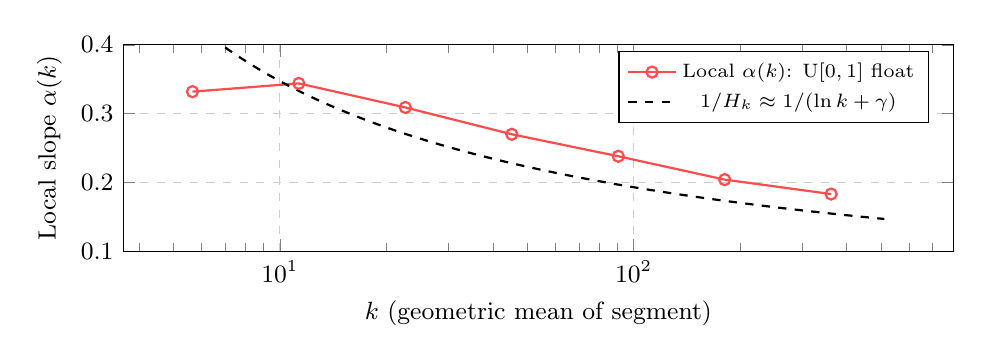
\begin{tikzpicture}
\begin{axis}[
  width=\columnwidth, height=4.2cm,
  xlabel={$k$ (geometric mean of segment)},
  ylabel={Local slope $\alpha(k)$},
  xmode=log,
  ymin=0.10, ymax=0.40,
  grid=major, grid style={dashed,gray!40},
  legend style={at={(0.97,0.97)},anchor=north east,font=\scriptsize},
  tick label style={font=\small}, label style={font=\small}
]
% Continuous weights: U[0,1] float (k=4..512)
\addplot[color=red!70,mark=o,mark size=2pt,thick]
  coordinates{
    (5.66, 0.332)(11.31, 0.344)(22.63, 0.309)(45.25, 0.270)
    (90.51, 0.238)(181.0, 0.204)(362.0, 0.183)};
\addlegendentry{Local $\alpha(k)$: $\mathrm{U}[0,1]$ float}
% Harmonic reference 1/H_k
\addplot[black,dashed,thick,domain=4:512,samples=60]
  {1/(ln(x)+0.5772)};
\addlegendentry{$1/H_k \approx 1/(\ln k + \gamma)$}
\end{axis}
\end{tikzpicture}
\caption{Local slope $\alpha(k)$ converges toward $1/H_k$ as $k$ grows,
consistent with the asymptotic skip\_ratio form $1-c/H_k$
(theory\_probe\_v4, $V=3{,}000$, continuous float weights).}
\label{fig:local_alpha}
\end{figure}

\noindent\textbf{Conjecture (two-regime model).}
The skip\_ratio of lazy-deletion Dijkstra on locally tree-like graphs is
consistent with a \emph{two-regime} empirical model:
\begin{equation}
\text{skip\_ratio}(k) \;\approx\;
\begin{cases}
  1 - c(F,W)\,/\,k^{\alpha(F,W)} & k \lesssim 100
    \quad\text{(power-law regime)} \\
  1 - A(F)\,/\,H_k & k \gg 100
    \quad\text{(harmonic regime)}
\end{cases}
\label{eq:tworegime}
\end{equation}
where $F$ denotes the weight distribution,
$\alpha(F,W)\in(0,0.32]$ is strongly associated with $\log(W_{\max}/W_{\min})$,
and $A(F)\to 1$ as $W\to\infty$ (the full i.i.d.\ harmonic limit).
Three caveats apply.
First, the crossover scale $k\approx 100$ is an \emph{approximate heuristic}:
the local slope decreases monotonically for all $k$ rather than
exhibiting a sharp regime boundary.
Second, $A(F)\to 1$ is an asymptotic statement; at $k=512$ we observe
push\_count$/V = 0.855\,H_{512}$, so the full harmonic limit
lies beyond our experimental range.
Third, bimodal distributions ($\alpha\approx 0$) are excluded; the
power-law form does not apply when one weight dominates BFS-like.
Formal derivation of the crossover scale and the functional form of
$\alpha(F,W)$ remain open problems.

\noindent\textbf{Practical implication.}
For the common engineering case of $k\leq 64$ with
$\mathrm{U}[1,100]$ weights, $\alpha\approx 0.27$--$0.29$ and
Equation~\eqref{eq:powerlaw} is accurate to within $\pm 0.025$
for $k\in[8,64]$ in skip\_ratio (max residual $0.022$ at $k=32$).
For wider $k$ ranges or other weight distributions,
Table~\ref{tab:alpha_vs_W} provides interpolation guidance.

% ──────────────────────────────────────────────────────────────────────
%  4. WHY NAIVE FIXES FAIL
% ──────────────────────────────────────────────────────────────────────
\section{Why Na\"ive Fixes Fail}
\label{sec:naivefixes}

A natural attempt to reduce skip\_ratio is to track how many times vertex
$v$ is currently in the heap (in\_heap[$v$]) and block a push when
in\_heap[$v$]\,$\geq\,\theta$.  We call this the \emph{threshold
heuristic} and evaluate it in Experiment~5.

\noindent\textbf{Correctness catastrophe.}
As shown in Table~\ref{tab:threshold}, $\theta=1$---which allows at most
one copy of each vertex in the heap---renders 53--74\% of vertices with
incorrect distances.  The mechanism is straightforward: blocking a push
creates a \emph{propagation gap}: if vertex $v$ is not re-pushed when its
tentative distance improves, its neighbors will never learn of the
improvement, cascading errors outward.  This is not a bug in the
heuristic; it is a structural property of lazy deletion.  The
``skip-on-pop'' strategy \emph{relies} on every relaxation being pushed
so that the minimum always surfaces correctly.

\begin{table}[t]
\centering
\caption{Threshold heuristic: accuracy vs.\ speedup (Experiment~5,
$V=1{,}000$, 5 random seeds).
$\theta=\infty$ is the unmodified baseline.}
\label{tab:threshold}
\small
\setlength{\tabcolsep}{4pt}
\begin{tabular}{cccccc}
\toprule
Graph & $\theta$ & Wrong nodes (\%) & Push reduc. & Time (ms) & Speedup \\
\midrule
\multirow{4}{*}{\shortstack{sparse\\$k=10$}}
 & $\infty$ & 0.0  & 0\%   & 3.69 & 1.00$\times$ \\
 & 3        & 5.3  & 6.7\% & 4.14 & 0.89$\times$ \\
 & 2        & 19.9 & 22.5\%& 3.38 & 1.09$\times$ \\
 & 1        & 53.3 & 52.9\%& 1.81 & 2.04$\times$ \\
\midrule
\multirow{4}{*}{\shortstack{dense-mid\\$k=32$}}
 & $\infty$ & 0.0  & 0\%   &11.07 & 1.00$\times$ \\
 & 3        & 17.9 & 20.3\%& 8.72 & 1.27$\times$ \\
 & 2        & 38.1 & 39.9\%& 6.54 & 1.69$\times$ \\
 & 1        & 69.0 & 66.8\%& 3.14 & 3.53$\times$ \\
\midrule
\multirow{4}{*}{\shortstack{dense-high\\$k=64$}}
 & $\infty$ & 0.0  & 0\%   &22.58 & 1.00$\times$ \\
 & 3        & 25.2 & 27.1\%&14.17 & 1.59$\times$ \\
 & 2        & 49.9 & 46.9\%& 9.32 & 2.42$\times$ \\
 & 1        & 74.3 & 71.6\%& 4.67 & 4.83$\times$ \\
\bottomrule
\end{tabular}
\end{table}

\noindent\textbf{No viable operating point.}
For sparse graphs ($k=10$), $\theta=3$ achieves only $0.89\times$
speedup (slower than baseline) while producing 5.3\% wrong nodes.  For
dense graphs, any $\theta\geq 2$ that yields noticeable speedup also
corrupts more than 18\% of answers.  There is no threshold at which
accuracy is acceptable and speedup is meaningful.

\noindent\textbf{Insight.}  The failure of the threshold heuristic
reveals that skip\_ratio is not a symptom of \emph{redundant} pushes---it
is an inherent cost of the lazy deletion protocol.  The correct remedy
is not to reduce pushes but to choose a data structure whose operational
semantics are compatible with the relaxation pattern.

\begin{figure}[t]
\centering
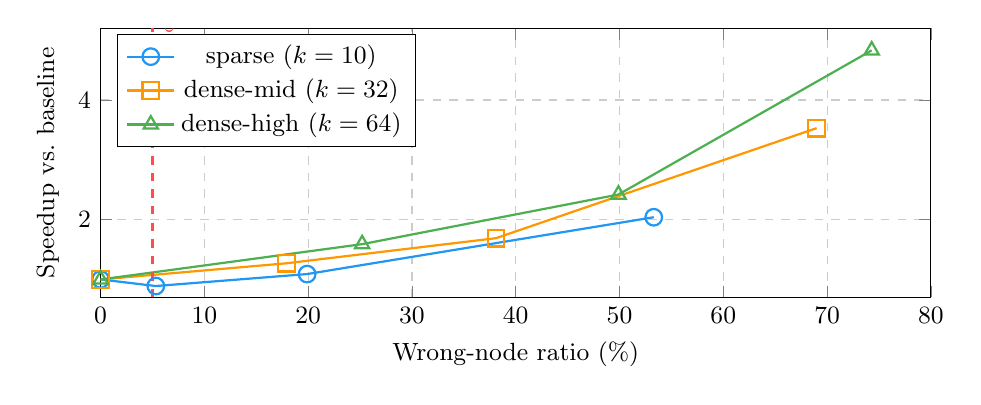
\begin{tikzpicture}
\begin{axis}[
  width=\columnwidth, height=5cm,
  xlabel={Wrong-node ratio (\%)},
  ylabel={Speedup vs.\ baseline},
  xmin=0, xmax=80, ymin=0.7, ymax=5.2,
  grid=major, grid style={dashed,gray!40},
  legend style={at={(0.02,0.98)},anchor=north west,font=\small},
  tick label style={font=\small}, label style={font=\small}
]
% sparse k=10
\addplot[heapqcolor,mark=o,mark size=3pt,thick]
  coordinates{(0,1.00)(5.32,0.89)(19.9,1.09)(53.3,2.04)};
\addlegendentry{sparse ($k=10$)}
% dense-mid k=32
\addplot[dialcolor,mark=square,mark size=3pt,thick]
  coordinates{(0,1.00)(17.9,1.27)(38.1,1.69)(69.0,3.53)};
\addlegendentry{dense-mid ($k=32$)}
% dense-high k=64
\addplot[fibcolor,mark=triangle,mark size=3pt,thick]
  coordinates{(0,1.00)(25.2,1.59)(49.9,2.42)(74.3,4.83)};
\addlegendentry{dense-high ($k=64$)}
% ideal accuracy boundary
\addplot[red!70,dashed,thick] coordinates{(5,0.7)(5,5.2)};
\node[font=\scriptsize,red!70,rotate=90] at (axis cs:6.5,4.5) {5\% error budget};
\end{axis}
\end{tikzpicture}
\caption{Threshold heuristic trade-off: wrong-node ratio vs.\ speedup
(Experiment~5, $V=1{,}000$).  Every point on each curve corresponds to a
different $\theta$ ($\infty,\,3,\,2,\,1$ from left to right).
No operating point meets a 5\% error budget with meaningful speedup.}
\label{fig:threshold}
\end{figure}

% ──────────────────────────────────────────────────────────────────────
%  5. DATA STRUCTURE COMPARISON
% ──────────────────────────────────────────────────────────────────────
\section{Data Structure Comparison}
\label{sec:comparison}

\subsection{Three-Way Comparison: Python and C++}

We compare three algorithms under identical graph conditions
(Experiments~6 and~7):
\begin{itemize}
  \item \textbf{heapq}: lazy deletion with Python's \texttt{heapq} /
        C++ \texttt{priority\_queue<>}.
  \item \textbf{Fibonacci}: decrease-key Dijkstra with a hand-crafted
        Fibonacci heap (Python and C++, same from-scratch implementation).
        Correctness verified by comparing distances against heapq output
        on all tested instances; maximum distance error is $0$ throughout.
  \item \textbf{Dial's}: circular bucket queue, integer weights $W=100$.
\end{itemize}

\noindent Table~\ref{tab:threeway} reports wall-clock times for $V=10{,}000$
in C++. Figure~\ref{fig:threeway} shows the corresponding bar chart.

\begin{table}[t]
\centering
\caption{Wall-clock time (ms) for $V=10{,}000$, 10 runs, C++ (Experiment~7).
All results verified correct ($\max\_\mathrm{err}=0$).}
\label{tab:threeway}
\small
\setlength{\tabcolsep}{5pt}
\begin{tabular}{lrrr}
\toprule
Graph condition & heapq & Fibonacci & Dial's \\
\midrule
sparse   ($k=8$)    & 4.54  & 10.29  & \textbf{1.06}  \\
dense-mid ($k=32$)  & 7.48  & 12.54  & \textbf{2.95}  \\
dense-high ($k=64$) & 9.51  & 14.29  & \textbf{4.28}  \\
\midrule
\multicolumn{4}{l}{\textit{Fibonacci / heapq ratio}} \\
sparse   & \multicolumn{3}{c}{$2.27\times$ slower} \\
dense-mid & \multicolumn{3}{c}{$1.68\times$ slower} \\
dense-high & \multicolumn{3}{c}{$1.50\times$ slower} \\
\midrule
\multicolumn{4}{l}{\textit{Dial's speedup over heapq}} \\
sparse   & \multicolumn{3}{c}{$4.28\times$ faster} \\
dense-mid & \multicolumn{3}{c}{$2.53\times$ faster} \\
dense-high & \multicolumn{3}{c}{$2.22\times$ faster} \\
\bottomrule
\end{tabular}
\end{table}

\begin{figure}[t]
\centering
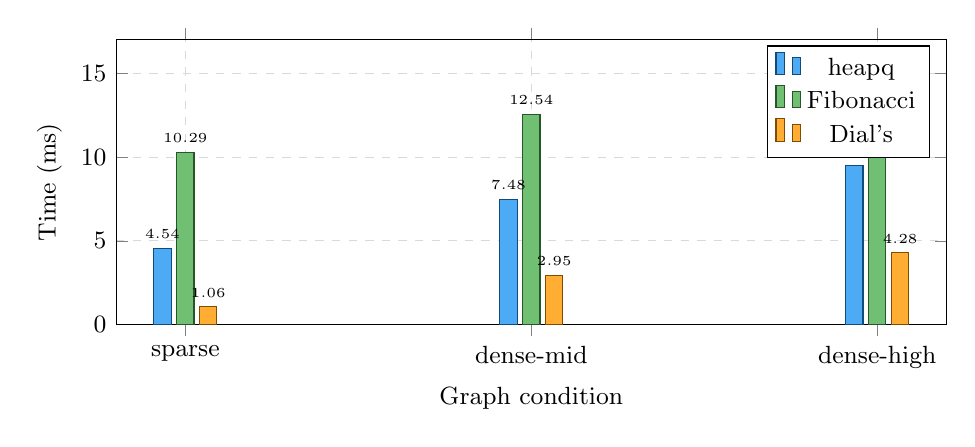
\begin{tikzpicture}
\begin{axis}[
  ybar,
  width=\columnwidth, height=5.2cm,
  bar width=0.22cm,
  symbolic x coords={sparse,dense-mid,dense-high},
  xtick=data,
  xlabel={Graph condition},
  ylabel={Time (ms)},
  legend style={at={(0.98,0.98)},anchor=north east,font=\small},
  tick label style={font=\small}, label style={font=\small},
  nodes near coords, nodes near coords align={vertical},
  every node near coord/.append style={font=\tiny},
  grid=major, grid style={dashed,gray!30},
  ymin=0, ymax=17
]
\addplot[fill=heapqcolor!80,draw=heapqcolor!50!black]
  coordinates{(sparse,4.54)(dense-mid,7.48)(dense-high,9.51)};
\addlegendentry{heapq}
\addplot[fill=fibcolor!80,draw=fibcolor!50!black]
  coordinates{(sparse,10.29)(dense-mid,12.54)(dense-high,14.29)};
\addlegendentry{Fibonacci}
\addplot[fill=dialcolor!80,draw=dialcolor!50!black]
  coordinates{(sparse,1.06)(dense-mid,2.95)(dense-high,4.28)};
\addlegendentry{Dial's}
\end{axis}
\end{tikzpicture}
\caption{C++ wall-clock time for $V=10{,}000$ (Experiment~7).
Dial's dominates across all densities; Fibonacci is consistently slowest.}
\label{fig:threeway}
\end{figure}

\noindent\textbf{Dial's speedup: peak vs.\ mean.}
Dial's delivers a \textbf{peak} speedup of $4.28\times$ over heapq in the
sparse C++ setting ($k=8$, $V=10{,}000$).  Across all three density
conditions ($k\in\{8,32,64\}$), the geometric mean speedup is
$\mathbf{2.9\times}$ in C++ and $\mathbf{1.5\times}$ in Python.  The
Python gap is narrower because the Python heap-push overhead (Python
object allocation) partially offsets the architectural advantage of Dial's
circular array.  Throughout the paper we report the C++ figures as the
language-independent performance bound and note Python figures where
relevant.

\noindent\textbf{Fibonacci heap: language-independent underperformance.}
In Python (Experiment~6), Fibonacci is $2.35\times$ slower than heapq for
$k=8$, $V=10{,}000$ (157\,ms vs.\ 67\,ms).  The C++ re-implementation
(Experiment~7) yields $2.27\times$ (10.3\,ms vs.\ 4.5\,ms)---essentially
the same ratio, confirming that the gap is \emph{not} a Python artifact.
The Python/C++ speedup is $14.8\times$ for heapq and $15.3\times$ for
Fibonacci, demonstrating that the language overhead is proportional for
both algorithms.  The Fibonacci underperformance therefore stems from
pointer-chasing and cache-unfriendly consolidation, not from interpreter
overhead.

\subsection{Dial's Natural Pruning Mechanism}
\label{sec:pruning}

To understand why Dial's achieves up to $4.28\times$ speedup, we
instrument its bucket operations in Experiment~8.

\noindent\textbf{Unprocessed pushes.}
Let $P$ denote total bucket pushes and $S$ denote stale skips.  In a
lazy deletion heap, $P = V + S$ (conservation), so every pushed entry
is either settled or skipped.  In Dial's, however, $P > V + S$: pushes
to future buckets beyond the maximum settled distance are \emph{never
popped at all}.  We call these \emph{unprocessed pushes} and denote
their fraction $\rho_{\mathrm{unp}} = (P - V - S)/P$.

\begin{figure}[t]
\centering
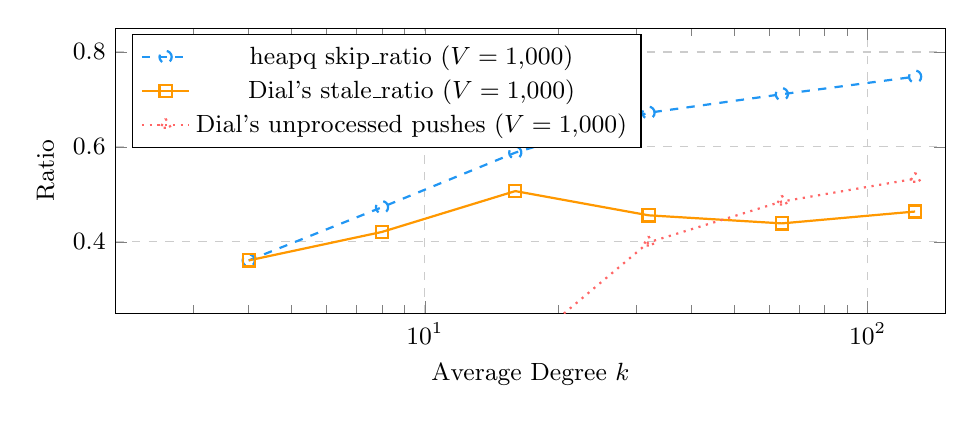
\begin{tikzpicture}
\begin{axis}[
  width=\columnwidth, height=5.2cm,
  xlabel={Average Degree $k$},
  ylabel={Ratio},
  xmin=2, xmax=150,
  ymin=0.25, ymax=0.85,
  xmode=log,
  grid=major, grid style={dashed,gray!40},
  legend style={at={(0.02,0.98)},anchor=north west,font=\small},
  tick label style={font=\small}, label style={font=\small}
]
% heapq skip_ratio V=1000
\addplot[heapqcolor,mark=o,mark size=2.2pt,thick,dashed]
  coordinates{(4,0.361)(8,0.473)(16,0.588)(32,0.672)(64,0.711)(128,0.748)};
\addlegendentry{heapq skip\_ratio ($V=1{,}000$)}

% Dial's stale_ratio V=1000
\addplot[dialcolor,mark=square,mark size=2.2pt,thick]
  coordinates{(4,0.361)(8,0.421)(16,0.507)(32,0.456)(64,0.439)(128,0.464)};
\addlegendentry{Dial's stale\_ratio ($V=1{,}000$)}

% unprocessed push fraction V=1000
\addplot[red!60,mark=triangle,mark size=2.2pt,thick,dotted]
  coordinates{(4,0.002)(8,0.091)(16,0.163)(32,0.399)(64,0.485)(128,0.533)};
\addlegendentry{Dial's unprocessed pushes ($V=1{,}000$)}
\end{axis}
\end{tikzpicture}
\caption{heapq skip\_ratio vs.\ Dial's stale\_ratio and unprocessed-push
fraction as functions of $k$ (Experiment~8, $V=1{,}000$, log $x$-axis).
As $k$ grows, heapq's skip\_ratio climbs monotonically while Dial's
stale\_ratio plateaus; the gap is absorbed by unprocessed pushes.}
\label{fig:stale}
\end{figure}

Figure~\ref{fig:stale} tells the story.  For $k=64$, heapq skip\_ratio is
0.711 and Dial's stale\_ratio is only 0.439---a difference of 0.272.  That
difference is accounted for by unprocessed pushes ($\rho_{\mathrm{unp}} =
0.485$): nearly \textbf{49\% of all Dial's pushes are never processed},
because the algorithm terminates once all $V$ nodes are settled, leaving
future-bucket entries abandoned.  By contrast, the binary heap must pop
every pushed entry.

The mechanism has an elegant explanation: in Dial's, settling node $u$ at
distance $d$ pushes its neighbors into buckets at $d + w$, some of which
may be far ahead of the current bucket pointer.  When the nearer of $u$'s
neighbors are settled later via better paths, those far-future entries
become both stale \emph{and} unreachable before the pointer reaches their
bucket.  Dense graphs ($k$ large) produce more such ``orphaned'' entries.
This is a qualitative advantage that binary heaps cannot replicate.

\subsection{Integer vs.\ Float Weights}

Experiment~9 repeats the Python and C++ comparison with float weights
$w\sim\mathcal{U}[0,1]$ (excluding Dial's, which requires integer
weights).  The relative ordering is unchanged: C++ Fibonacci is
$1.6$--$2.7\times$ slower than heapq at $V=10{,}000$, and the Python/C++
ratio is $15\times$ for both algorithms.  We conclude that the performance
relationship between heapq and Fibonacci heap is \textbf{independent of
weight type}, generalizing our findings beyond integer graphs.

\subsection{Data-Structure Selection Framework}
\label{sec:framework}

\noindent\textbf{Effect of maximum edge weight $W$ (Experiment~B).}
All prior comparisons used $W{=}100$.  Experiment~B varies $W\in\{100,\,500,\,1{,}000,\,5{,}000,\,10{,}000\}$
with $V{=}10{,}000$ fixed to characterize the interaction between $W$ and
Dial's speedup.  For sparse graphs ($k{=}8$), Dial's advantage erodes
sharply: speedup is $2.85\times$ at $W{=}1{,}000$ but falls to $0.80\times$
at $W{=}5{,}000$ and $0.66\times$ at $W{=}10{,}000$, placing the
breakeven threshold $W^{*}$ in the range $[1{,}000,\,5{,}000]$ for this
setting (the measured points bracket the crossover; precise location
requires finer $W$ sampling).  For denser
graphs ($k{\geq}32$), Dial's remains faster than heapq even at $W{=}10{,}000$
(${\geq}1.07\times$ speedup), so $W^{*}{>}10{,}000$ in this regime.  The
mechanism is the circular-array traversal cost: with $W{+}1$ buckets,
the number of bucket-scan iterations grows proportionally to $W$, eventually
dominating the $O(E\log E)$ savings.

Table~\ref{tab:framework} consolidates our findings into actionable
guidance.  The decision depends on two observable graph properties:
weight type and average degree $k$.

\begin{table}[t]
\centering
\caption{Data-structure selection framework.
$k_{\mathrm{low}}\approx 10$ separates regimes where skip\_ratio $<0.5$.
$W^{*}$ is the maximum edge weight below which Dial's beats heapq
(Experiment~B; $V{=}10{,}000$).}
\label{tab:framework}
\small
\renewcommand{\arraystretch}{1.2}
\begin{tabular}{p{2.3cm}p{1.5cm}p{3.5cm}}
\toprule
\textbf{Condition} & \textbf{Recommended} & \textbf{Rationale} \\
\midrule
Integer weights, any $k$, $W \leq W^{*}$\,\textsuperscript{\dag} &
  Dial's bucket queue &
  Up to $4\times$ speedup (sparse) via natural pruning; O$(V{+}E{+}W)$. \\
\addlinespace
Integer weights, $k{=}8$, $W \gtrsim 5{,}000$ &
  heapq &
  Dial's speedup $< 1$ at $W{=}5{,}000$ ($0.80\times$) and $0.66\times$
  at $W{=}10{,}000$; circular-array traversal dominates. \\
\addlinespace
Float weights, $k \leq 10$ (sparse) &
  heapq (lazy deletion) &
  skip\_ratio $<0.5$; overhead acceptable; simplest implementation. \\
\addlinespace
Float weights, $k > 10$ (dense) &
  heapq (lazy deletion) &
  Fibonacci does not outperform heapq even in C++; no benefit to switch. \\
\addlinespace
Fibonacci heap &
  Avoid in practice &
  $1.5$--$2.3\times$ slower than heapq in C++ due to pointer-chasing;
  theoretical O$(V\log V{+}E)$ advantage is not realized. \\
\bottomrule
\multicolumn{3}{p{7.3cm}}{\textsuperscript{\dag}\small
  $W^{*}$ depends on $k$: for $k{=}8$, $W^{*}\in[1{,}000,\,5{,}000]$
  (crossover observed between these measured values);
  for $k{\geq}32$, Dial's remains faster even at $W{=}10{,}000$
  (${\geq}1.07\times$ speedup), so $W^{*}{>}10{,}000$ in this regime.
  See Section~\ref{sec:framework}.}
\end{tabular}
\end{table}

% ──────────────────────────────────────────────────────────────────────
%  6. REAL-WORLD VALIDATION
% ──────────────────────────────────────────────────────────────────────
\section{Real-World Validation}
\label{sec:realworld}

We test formula~\eqref{eq:powerlaw} on three SNAP~\cite{snapnets}
datasets.  Integer weights $w\sim\mathcal{U}_{\mathbb{Z}}[1,100]$ are
assigned randomly (seed 42); skip\_ratio is averaged over 10 random source
vertices.  Results appear in Table~\ref{tab:realworld} and
Figure~\ref{fig:overlay}.

\begin{table}[t]
\centering
\caption{Formula validation on SNAP real-world graphs (Experiment~10).}
\label{tab:realworld}
\small
\setlength{\tabcolsep}{4pt}
\begin{tabular}{lrrrrr}
\toprule
Dataset & $V$ & $E$ & $k$ & Measured & Predicted \\
 & & & & skip\_ratio & (Eq.~\ref{eq:powerlaw}) \\
\midrule
ego-Facebook  & 4,039    & 88,234    & 43.7 & 0.655 & 0.671 \\
ca-GrQc       & 5,241    & 14,484    & 5.5  & 0.335 & 0.435 \\
roadNet-CA    & 1,965,206& 2,766,607 & 2.8  & 0.116 & 0.326 \\
\midrule
 & & & \multicolumn{2}{c}{Relative error} & \\
\cmidrule(lr){4-6}
ego-Facebook  & & & & \multicolumn{2}{c}{\textbf{2.5\%}} \\
ca-GrQc       & & & & \multicolumn{2}{c}{23.1\%} \\
roadNet-CA    & & & & \multicolumn{2}{c}{64.4\%} \\
\bottomrule
\end{tabular}
\end{table}

\begin{figure}[t]
\centering
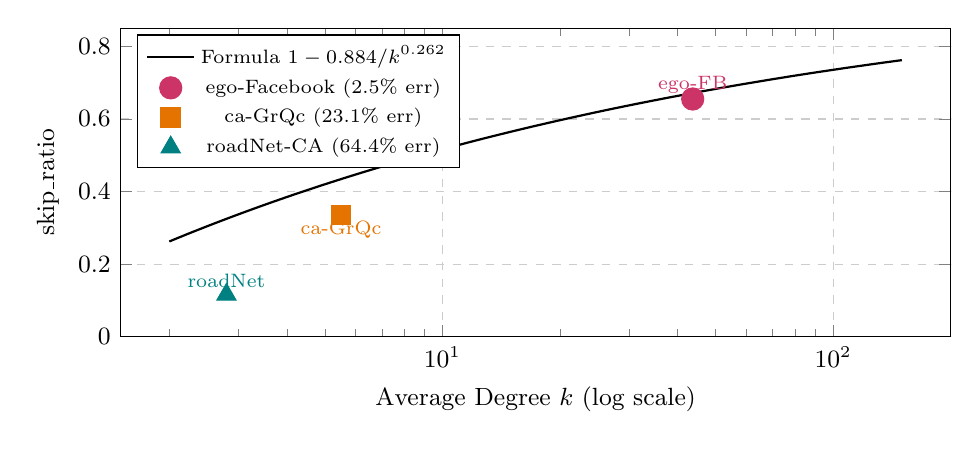
\begin{tikzpicture}
\begin{axis}[
  width=\columnwidth, height=5.5cm,
  xlabel={Average Degree $k$ (log scale)},
  ylabel={skip\_ratio},
  xmin=1.5, xmax=200,
  ymin=0, ymax=0.85,
  xmode=log,
  grid=major, grid style={dashed,gray!40},
  legend style={at={(0.02,0.98)},anchor=north west,font=\scriptsize},
  tick label style={font=\small}, label style={font=\small}
]
% power law curve
\addplot[thick,black,domain=2:150,samples=80]
  {1 - 0.884*x^(-0.262)};
\addlegendentry{Formula $1-0.884/k^{0.262}$}

% ego-Facebook (good fit)
\addplot[color=purple!80,mark=*,mark size=4pt,only marks]
  coordinates{(43.7, 0.655)};
\addlegendentry{ego-Facebook (2.5\% err)}

% ca-GrQc (moderate)
\addplot[color=orange!90!black,mark=square*,mark size=3.5pt,only marks]
  coordinates{(5.5, 0.335)};
\addlegendentry{ca-GrQc (23.1\% err)}

% roadNet-CA (large deviation)
\addplot[color=teal,mark=triangle*,mark size=4pt,only marks]
  coordinates{(2.8, 0.116)};
\addlegendentry{roadNet-CA (64.4\% err)}

% Annotations
\node[font=\scriptsize,purple!80] at (axis cs:43.7,0.695) {ego-FB};
\node[font=\scriptsize,orange!90!black] at (axis cs:5.5,0.295) {ca-GrQc};
\node[font=\scriptsize,teal] at (axis cs:2.8,0.155) {roadNet};
\end{axis}
\end{tikzpicture}
\caption{skip\_ratio formula validated on SNAP datasets (Experiment~10).
Black curve: formula~\eqref{eq:powerlaw} fitted on random graphs.
Colored markers: measured skip\_ratio on real graphs.}
\label{fig:overlay}
\end{figure}

\noindent\textbf{ego-Facebook (2.5\% error).}
This dense social network ($k=43.7$) closely resembles an
Erd\H{o}s--R\'enyi graph: high average degree, low clustering relative
to $k$, and short cycles of length $\geq 4$.  The locally tree-like
assumption holds approximately, and the formula achieves 2.5\% relative
error---well within experimental noise.

\noindent\textbf{ca-GrQc (23.1\% error).}
The Arxiv collaboration network has $k=5.5$, placing it at the left tail
of the power-law curve.  The error has two separable components.
\emph{Small-$k$ component:} even on an ER random graph at $k\approx 5.5$,
the formula carries $\Delta\approx 2$--$4\%$ inaccuracy (by interpolation
from the $k=4$ under-prediction of $\Delta\approx 0.03$); this accounts
for roughly $2$--$4$ percentage points of the 23\% gap.
\emph{Structural component:} collaboration networks exhibit high clustering
(many short cycles), violating the tree-like assumption on which the
formula rests; the residual $\approx 19$--$21\%$ error is attributable to
this structural mismatch.  The two effects are therefore roughly 1:7 in magnitude.

\noindent\textbf{roadNet-CA (64.4\% error).}
This is not a limitation of the formula but is \emph{consistent with
the scope of its derivation}.  Road networks are planar graphs (bounded genus, no
long-range edges); their average degree $k=2.8$ is far below the range
for which the locally tree-like assumption holds, and their structure
introduces long-range correlations in settling order.  Measured
skip\_ratio is 0.116 vs.\ predicted 0.326---road networks exhibit
markedly \emph{less} heap waste than random graphs of the same degree
because most paths are monotone along road corridors.  Applying
formula~\eqref{eq:powerlaw} to planar graphs would be a misuse; we treat
the deviation as confirmation that the formula's applicability boundary
is correctly identified by the locally tree-like condition.

\noindent\textbf{Scale-free (Barab\'{a}si--Albert) graphs (Experiment C).}
Real social and technological networks often follow a power-law degree
distribution rather than the Poisson distribution of Erd\H{o}s--R\'{e}nyi
graphs.  We test formula~\eqref{eq:powerlaw} on Barab\'{a}si--Albert (BA)
graphs~\cite{barabasi1999} with attachment parameter $m\in\{4,8,16,32\}$
(expected $k_{\mathrm{avg}}=2m\in\{8,16,32,64\}$), $V\in\{1{,}000,\,10{,}000\}$,
random integer weights, and 10 repetitions per configuration.

The formula generalizes well to scale-free structure: at
$k_{\mathrm{avg}}\geq 16$, relative error is $2$--$4\%$ for both BA and ER
graphs---essentially indistinguishable.  At $k_{\mathrm{avg}}\approx 8$
(sparse), BA graphs show a modestly lower skip\_ratio ($\approx 0.450$) than
ER graphs with matching $k_{\mathrm{avg}}$ ($\approx 0.487$), yielding
$7$--$8\%$ relative error instead of $<6\%$.  The gap is attributable to
degree heterogeneity in BA graphs: hub nodes (high-degree) are settled
early and generate fewer subsequent relaxations per unit of $k_{\mathrm{avg}}$,
slightly reducing the stale-pop fraction.  Nonetheless, the formula provides
a useful first approximation for scale-free graphs, extending its applicability
beyond Erd\H{o}s--R\'enyi random graphs.

% ──────────────────────────────────────────────────────────────────────
%  7. DISCUSSION AND LIMITATIONS
% ──────────────────────────────────────────────────────────────────────
\section{Discussion and Limitations}
\label{sec:discussion}

\noindent\textbf{Scope of validity.}
Formula~\eqref{eq:powerlaw} is calibrated on Erd\H{o}s--R\'enyi-like
random graphs with uniform edge weights.  It generalizes to dense social
networks (ego-Facebook, 2.5\% error) but not to planar or hierarchical
graphs.  For structured inputs, the skip\_ratio can be substantially
lower than the formula predicts, as roadNet-CA demonstrates.  A
practitioner should verify that their target graph exhibits high average
degree and low local clustering before applying the formula.

\noindent\textbf{Fibonacci heap: theoretical vs.\ practical optimality.}
The Fibonacci heap achieves the theoretically optimal O$(V\log V + E)$
bound, yet our C++ measurements show it is $1.5$--$2.3\times$ slower
than a binary heap for $V\leq 10{,}000$ across all tested densities.
This gap is language-independent---we replicate it in both Python and C++
with the same ratio---and stems from pointer-chasing overheads during
consolidation and cascading cuts.  For graphs where $E\gg V\log V$
(i.e., extremely dense), the Fibonacci heap's asymptotic advantage might
eventually manifest, but such densities exceed the range studied here.
We recommend against Fibonacci heaps unless theoretical guarantees are
mandated by a formal proof system.

\noindent\textbf{Indexed and $d$-ary heaps (supplemental experiment).}
To probe the two most commonly suggested alternatives to lazy binary heapq,
we ran a Python supplemental experiment (\texttt{dijkstra\_heap\_compare.py})
across $V\in\{500,1000,3000,5000,10000\}$ and $k\in\{4,8,16,32,64,128\}$
with five repetitions each ($\mathrm{U}[1,100]$).
\emph{Hardware note:} this experiment ran on a local MacBook Pro (Apple M3,
macOS), not on the GCP e2-standard-4 instance used for the main experiments;
timing comparisons within this experiment are internally consistent, but
cross-experiment absolute times should not be compared directly.

\textit{Skip-ratio is implementation-invariant.}
All three lazy-deletion variants (binary, 4-ary, 8-ary heaps) produced
skip\_ratios within $\pm 0.001$ of each other at every $(V,k)$ point
($V=3{,}000$ representative values: $0.242$, $0.438$, $0.573$, $0.660$,
$0.711$, $0.746$ for $k=4,8,16,32,64,128$).
As expected, the \emph{indexed} binary heap achieves skip\_ratio$\,=0$
by maintaining a position array for O(log $V$) decrease-key.

\textit{Lazy binary heapq vs.\ indexed heap (Python).}
Despite zero skip overhead, the indexed heap is consistently \emph{slower}
than lazy heapq for $k\leq 32$: speedup (indexed$/$lazy) ranges from
$3.4\times$ at $k=4$ to $1.5\times$ at $k=32$ ($V=10{,}000$),
because each decrease-key requires a random-access position lookup and
upward sift, whereas heapq's lazy push is a simple append.
The gap closes near $k\approx 64$--$128$ (speedup $\approx 1.0$),
where the high skip\_ratio ($\approx70$--$75\%$) begins to offset indexed
heap's bookkeeping cost.  These Python results corroborate the
$1.5\times$ geometric-mean speedup of lazy heapq reported in
Section~\ref{sec:comparison}.

\textit{$d$-ary heaps (Python).}
4-ary and 8-ary lazy heaps are uniformly \emph{slower} than binary heapq
across all $(V,k)$ configurations tested.  The extra branching factor
reduces tree height but adds per-level comparison work with no cache
benefit in Python's interpreted loop; the slowdown versus binary ranges
from $1.2\times$ at $k=4$ to $1.7\times$ at $k=64$.  In optimized
C++, $d$-ary heaps can outperform binary heaps due to SIMD-friendly
child comparisons~\cite{ahuja1993}; extending the C++ benchmark to $d$-ary
heaps is a natural next step.
\emph{Pairing heaps} offer favorable amortized decrease-key and have not been
characterized under lazy deletion; extending the selection framework to
them remains open.

\noindent\textbf{Statistical note.}
Main experiments (Sections~\ref{sec:analysis}--\ref{sec:comparison}) use
5--10 repetitions per $(V,k)$ configuration and report means.
The observed inter-run variation is $\leq 0.013$ in skip\_ratio across
all $(V,k)$ pairs (Table~\ref{tab:vindependence}), indicating high stability.
Weight-distribution experiments (Section~\ref{sec:weightdist}) use
30 repetitions ($V=3{,}000$).

\noindent\textbf{Source-vertex sensitivity.}
All main experiments use source vertex~0 (seed~42).  To verify that this
design choice does not inflate or suppress the measured skip\_ratio, we
ran a supplementary experiment sampling 20 uniformly random source
vertices across 5 graph instances, for $V\in\{1{,}000,\,3{,}000,\,10{,}000\}$
and $k\in\{4,8,16,32,64,128\}$ ($\mathrm{U}[1,100]$).
The coefficient of variation of skip\_ratio across sources is at most
$2.6\%$ (at $V=1{,}000$, $k=4$, where skip\_ratio is smallest) and falls
below $0.5\%$ for $k\geq 64$.
Standard deviation across sources does not exceed $0.009$ at any $(V,k)$
tested.  We conclude that skip\_ratio is effectively source-independent for
the ER-like graphs studied here, consistent with the locally tree-like
theory (the expected push count per vertex depends only on local degree
structure, not on which vertex is the source).

\noindent\textbf{Future work.}
Three open questions arise naturally from this study:
\begin{enumerate}
  \item \emph{Theoretical derivation of the two-regime empirical model.}
        Section~\ref{sec:weightdist} establishes empirically that the
        local slope $\alpha(k)$ converges toward $1/H_k$ and that the
        push\_count$/V$ ratio approaches $H_k$ from below as $k\to\infty$.
        A formal proof connecting the record-minimum process on
        Poisson--Galton--Watson trees to both the power-law regime and the
        harmonic limit---and a derivation of the crossover scale
        $k\approx 100$---remains open.
  \item \emph{Exact characterization of $\alpha(F,W)$.}
        The dependence $\alpha\approx f(\log(W_{\max}/W_{\min}))$
        is empirically clear but analytically unproven.  An exact formula
        for the functional $\alpha(F,W)$ and its limiting value under
        continuous distributions would close this gap.
  \item \emph{Structured-graph models.}  The 64\% error on roadNet-CA
        motivates a separate characterization of skip\_ratio for planar and
        hierarchical graphs, which have known algebraic structure amenable
        to analytic approaches.
\end{enumerate}

% ──────────────────────────────────────────────────────────────────────
%  8. CONCLUSION
% ──────────────────────────────────────────────────────────────────────
\section{Conclusion}
\label{sec:conclusion}

We have presented a systematic empirical characterization of the
lazy deletion overhead in Dijkstra's algorithm as a closed-form function
of graph structure, filling a gap in prior experimental surveys that
treat this overhead as a fixed implementation detail.  Our key findings are:

\begin{enumerate}
  \item \textbf{Power-law skip\_ratio, V-independent.}
        $\text{skip\_ratio}(k)\approx 1-0.884/k^{0.262}$ ($R^2=0.984$)
        holds across graph sizes from 500 to $10^6$ vertices, confirming
        that skip\_ratio is primarily determined by average degree $k$
        under fixed weight distribution and ER-like graph topology.
        The formula generalizes to Barab\'{a}si--Albert scale-free graphs
        with $<8\%$ relative error (Experiment~C).
  \item \textbf{Two-regime empirical model and weight-distribution dependence.}
        The exponent $\alpha$ is not universal: it is strongly associated with
        $\log(W_{\max}/W_{\min})$ and ranges from $0$ (constant weights)
        to ${\approx}0.32$ (continuous uniform, $k\leq 64$).
        At larger $k$, the local slope converges toward $1/H_k$,
        revealing that the power-law regime transitions to a harmonic
        regime $1-A/H_k$ as $k\to\infty$---consistent with the
        classical i.i.d.\ record-minimum bound and never violating it.
  \item \textbf{Threshold fixes are broken.}
        Push-blocking heuristics cause propagation gaps corrupting up to
        74\% of shortest distances at any setting that yields measurable
        speedup.
  \item \textbf{Fibonacci heap is not practical.}
        Despite O$(V\log V + E)$, Fibonacci heap is $1.5$--$2.3\times$
        slower than heapq in optimized C++, language- and
        density-independent.
  \item \textbf{Dial's natural pruning delivers $4\times$ peak speedup.}
        Up to 49\% of Dial's bucket pushes are never processed---a
        structural property with no binary-heap analog---enabling
        \textbf{peak $4.3\times$} speedup for sparse integer-weight graphs
        and a geometric mean of $2.9\times$ in C++ ($1.5\times$ in Python).
\end{enumerate}

The practical takeaway is:
\emph{skip\_ratio is a tight function of average degree $k$ and weight
distribution; matching graph structure to the right priority queue via
our selection framework achieves up to $4.3\times$ peak speedup.}
Specifically: use Dial's for sparse integer weights ($W \lesssim 1{,}000$
for $k{=}8$; any $W$ for $k{\geq}32$), heapq for float weights or large
$W$, and avoid Fibonacci heaps in practice.

% ──────────────────────────────────────────────────────────────────────
%  REFERENCES
% ──────────────────────────────────────────────────────────────────────
\bibliographystyle{IEEEtran}
\begin{thebibliography}{10}

\bibitem{dijkstra1959}
E.~W. Dijkstra,
``A note on two problems in connexion with graphs,''
\emph{Numerische Mathematik}, vol.~1, no.~1, pp.~269--271, 1959.

\bibitem{fredman1987}
M.~L. Fredman and R.~E. Tarjan,
``Fibonacci heaps and their uses in improved network optimization
algorithms,''
\emph{Journal of the ACM}, vol.~34, no.~3, pp.~596--615, 1987.

\bibitem{dial1969}
R.~B. Dial,
``Algorithm 360: Shortest-path forest with topological ordering,''
\emph{Communications of the ACM}, vol.~12, no.~11, pp.~632--633, 1969.

\bibitem{goldberg2005}
A.~V. Goldberg, H.~Kaplan, and R.~F. Werneck,
``Better landmarks within reach,''
in \emph{Proc.\ Workshop on Experimental Algorithms (WEA)}, 2007,
pp.~38--51.

\bibitem{sanders2005}
P.~Sanders and D.~Schultes,
``Highway hierarchies hasten exact shortest path queries,''
in \emph{Proc.\ ESA}, 2005, pp.~568--579.

\bibitem{chen2007}
M.~Chen, E.~Felsner, and A.~Schulz,
``On the performance of priority queues for shortest path algorithms,''
in \emph{Proc.\ ALENEX}, 2007, pp.~52--63.

\bibitem{cherkassky1996}
B.~V. Cherkassky, A.~V. Goldberg, and T.~Radzik,
``Shortest paths algorithms: Theory and experimental evaluation,''
\emph{Mathematical Programming}, vol.~73, pp.~129--174, 1996.

\bibitem{larkin2014}
D.~H. Larkin, S.~Sen, and R.~E. Tarjan,
``A back-to-basics empirical study of priority queues,''
in \emph{Proc.\ ALENEX}, 2014, pp.~61--72.

\bibitem{bollobas2001}
B. Bollob\'as,
\emph{Random Graphs}, 2nd~ed.
Cambridge University Press, 2001.

\bibitem{barabasi1999}
A.-L. Barab\'asi and R. Albert,
``Emergence of scaling in random networks,''
\emph{Science}, vol.~286, pp.~509--512, 1999.

\bibitem{flajolet2009analytic}
P.~Flajolet and R.~Sedgewick,
\emph{Analytic Combinatorics}.
Cambridge University Press, 2009.

\bibitem{snapnets}
J.~Leskovec and A.~Krevl,
``{SNAP Datasets}: {Stanford} Large Network Dataset Collection,''
\url{http://snap.stanford.edu/data}, Jun. 2014.

\bibitem{ahuja1993}
R.~K. Ahuja, T.~L. Magnanti, and J.~B. Orlin,
\emph{Network Flows: Theory, Algorithms, and Applications}.
Prentice Hall, 1993.

\bibitem{demetrescu2006}
C.~Demetrescu, A.~V. Goldberg, and D.~S. Johnson, Eds.,
\emph{The Shortest Path Problem: Ninth DIMACS Implementation Challenge},
vol.~74, DIMACS Series in Discrete Mathematics and Theoretical Computer
Science.  American Mathematical Society, 2009.

\end{thebibliography}

\end{document}
